% This file was created by matlab2tikz.
%
\definecolor{mycolor1}{rgb}{0.06600,0.44300,0.74500}%
\definecolor{mycolor2}{rgb}{0.12941,0.12941,0.12941}%
\definecolor{mycolor3}{rgb}{0.86600,0.32900,0.00000}%
\definecolor{mycolor4}{rgb}{0.92900,0.69400,0.12500}%
\definecolor{mycolor5}{rgb}{0.52100,0.08600,0.81900}%
\definecolor{mycolor6}{rgb}{0.23100,0.66600,0.19600}%
\definecolor{mycolor7}{rgb}{0.18400,0.74500,0.93700}%
\definecolor{mycolor8}{rgb}{0.81900,0.01500,0.54500}%
%
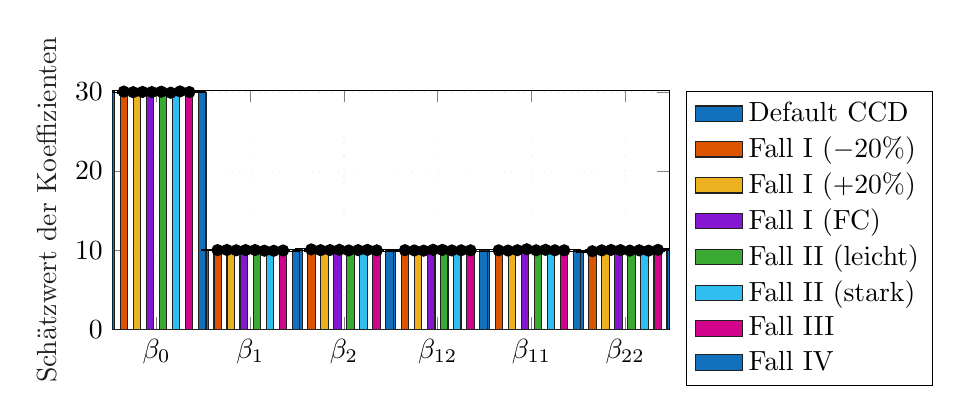
\begin{tikzpicture}

\begin{axis}[%
width=0.583\textwidth,
height=0.25\textwidth,
at={(0\textwidth,0\textwidth)},
scale only axis,
bar shift auto,
xmin=0.5300,
xmax=6.4700,
xtick={1.0000,2.0000,3.0000,4.0000,5.0000,6.0000},
xticklabels={{$\beta_0$},{$\beta_1$},{$\beta_2$},{$\beta_{12}$},{$\beta_{11}$},{$\beta_{22}$}},
ymin=0.0000,
ymax=30.1738,
ylabel style={font=\color{mycolor2}},
ylabel={Schätzwert der Koeffizienten},
axis background/.style={fill=white},
xmajorgrids,
ymajorgrids,
grid style={dotted, opacity=0.25},
legend style={at={(1.03,1)}, anchor=north west, legend cell align=left, align=left}
]
\addplot[ybar, bar width=0.08, fill=mycolor1, draw=mycolor2, area legend] table[row sep=crcr] {%
1.0000	30.0481\\
2.0000	10.0064\\
3.0000	10.0957\\
4.0000	10.0006\\
5.0000	9.9805\\
6.0000	9.8686\\
};
\addplot[forget plot, color=mycolor2] table[row sep=crcr] {%
0.5300	0.0000\\
6.4700	0.0000\\
};
\addlegendentry{Default CCD}

\addplot[ybar, bar width=0.08, fill=mycolor3, draw=mycolor2, area legend] table[row sep=crcr] {%
1.0000	29.9734\\
2.0000	10.0250\\
3.0000	9.9999\\
4.0000	9.9632\\
5.0000	9.9502\\
6.0000	9.9766\\
};
\addplot[forget plot, color=mycolor2] table[row sep=crcr] {%
0.5300	0.0000\\
6.4700	0.0000\\
};
\addlegendentry{Fall I ($-20\%$)}

\addplot[ybar, bar width=0.08, fill=mycolor4, draw=mycolor2, area legend] table[row sep=crcr] {%
1.0000	30.0057\\
2.0000	9.9860\\
3.0000	10.0170\\
4.0000	9.9388\\
5.0000	9.9924\\
6.0000	10.0287\\
};
\addplot[forget plot, color=mycolor2] table[row sep=crcr] {%
0.5300	0.0000\\
6.4700	0.0000\\
};
\addlegendentry{Fall I ($+20\%$)}

\addplot[ybar, bar width=0.08, fill=mycolor5, draw=mycolor2, area legend] table[row sep=crcr] {%
1.0000	29.9896\\
2.0000	10.0133\\
3.0000	10.0472\\
4.0000	10.0486\\
5.0000	10.1194\\
6.0000	10.0049\\
};
\addplot[forget plot, color=mycolor2] table[row sep=crcr] {%
0.5300	0.0000\\
6.4700	0.0000\\
};
\addlegendentry{Fall I (FC)}

\addplot[ybar, bar width=0.08, fill=mycolor6, draw=mycolor2, area legend] table[row sep=crcr] {%
1.0000	30.0319\\
2.0000	10.0178\\
3.0000	9.9674\\
4.0000	10.0365\\
5.0000	9.9828\\
6.0000	9.9442\\
};
\addplot[forget plot, color=mycolor2] table[row sep=crcr] {%
0.5300	0.0000\\
6.4700	0.0000\\
};
\addlegendentry{Fall II (leicht)}

\addplot[ybar, bar width=0.08, fill=mycolor7, draw=mycolor2, area legend] table[row sep=crcr] {%
1.0000	29.9064\\
2.0000	9.9360\\
3.0000	10.0035\\
4.0000	9.9668\\
5.0000	10.0435\\
6.0000	9.9815\\
};
\addplot[forget plot, color=mycolor2] table[row sep=crcr] {%
0.5300	0.0000\\
6.4700	0.0000\\
};
\addlegendentry{Fall II (stark)}

\addplot[ybar, bar width=0.08, fill=mycolor8, draw=mycolor2, area legend] table[row sep=crcr] {%
1.0000	30.0693\\
2.0000	9.9229\\
3.0000	10.0336\\
4.0000	9.9818\\
5.0000	9.9860\\
6.0000	9.9383\\
};
\addplot[forget plot, color=mycolor2] table[row sep=crcr] {%
0.5300	0.0000\\
6.4700	0.0000\\
};
\addlegendentry{Fall III}

\addplot[ybar, bar width=0.08, fill=mycolor1, draw=mycolor2, area legend] table[row sep=crcr] {%
1.0000	29.9864\\
2.0000	9.9586\\
3.0000	9.9781\\
4.0000	9.9826\\
5.0000	9.9840\\
6.0000	10.0401\\
};
\addplot[forget plot, color=mycolor2] table[row sep=crcr] {%
0.5300	0.0000\\
6.4700	0.0000\\
};
\addlegendentry{Fall IV}

\addplot [color=black, line width=0.4pt, only marks, forget plot]
 plot [error bars/.cd, y dir=both, y explicit, error bar style={line width=0.4pt}, error mark options={line width=0.4pt, mark size=6.0pt, rotate=90}]
 table[row sep=crcr, y error plus index=2, y error minus index=3]{%
0.6500	30.0481	0.1044	0.1044\\
1.6500	10.0064	0.1032	0.1032\\
2.6500	10.0957	0.1045	0.1045\\
3.6500	10.0006	0.1084	0.1084\\
4.6500	9.9805	0.1048	0.1048\\
5.6500	9.8686	0.1039	0.1039\\
};
\addplot [color=black, line width=0.4pt, only marks, forget plot]
 plot [error bars/.cd, y dir=both, y explicit, error bar style={line width=0.4pt}, error mark options={line width=0.4pt, mark size=6.0pt, rotate=90}]
 table[row sep=crcr, y error plus index=2, y error minus index=3]{%
0.7500	29.9734	0.1039	0.1039\\
1.7500	10.0250	0.1042	0.1042\\
2.7500	9.9999	0.1040	0.1040\\
3.7500	9.9632	0.1089	0.1089\\
4.7500	9.9502	0.1045	0.1045\\
5.7500	9.9766	0.1048	0.1048\\
};
\addplot [color=black, line width=0.4pt, only marks, forget plot]
 plot [error bars/.cd, y dir=both, y explicit, error bar style={line width=0.4pt}, error mark options={line width=0.4pt, mark size=6.0pt, rotate=90}]
 table[row sep=crcr, y error plus index=2, y error minus index=3]{%
0.8500	30.0057	0.1049	0.1049\\
1.8500	9.9860	0.1039	0.1039\\
2.8500	10.0170	0.1028	0.1028\\
3.8500	9.9388	0.1110	0.1110\\
4.8500	9.9924	0.1021	0.1021\\
5.8500	10.0287	0.1043	0.1043\\
};
\addplot [color=black, line width=0.4pt, only marks, forget plot]
 plot [error bars/.cd, y dir=both, y explicit, error bar style={line width=0.4pt}, error mark options={line width=0.4pt, mark size=6.0pt, rotate=90}]
 table[row sep=crcr, y error plus index=2, y error minus index=3]{%
0.9500	29.9896	0.1041	0.1041\\
1.9500	10.0133	0.1057	0.1057\\
2.9500	10.0472	0.1034	0.1034\\
3.9500	10.0486	0.1102	0.1102\\
4.9500	10.1194	0.1069	0.1069\\
5.9500	10.0049	0.1042	0.1042\\
};
\addplot [color=black, line width=0.4pt, only marks, forget plot]
 plot [error bars/.cd, y dir=both, y explicit, error bar style={line width=0.4pt}, error mark options={line width=0.4pt, mark size=6.0pt, rotate=90}]
 table[row sep=crcr, y error plus index=2, y error minus index=3]{%
1.0500	30.0319	0.1038	0.1038\\
2.0500	10.0178	0.1037	0.1037\\
3.0500	9.9674	0.1039	0.1039\\
4.0500	10.0365	0.1084	0.1084\\
5.0500	9.9828	0.1032	0.1032\\
6.0500	9.9442	0.1038	0.1038\\
};
\addplot [color=black, line width=0.4pt, only marks, forget plot]
 plot [error bars/.cd, y dir=both, y explicit, error bar style={line width=0.4pt}, error mark options={line width=0.4pt, mark size=6.0pt, rotate=90}]
 table[row sep=crcr, y error plus index=2, y error minus index=3]{%
1.1500	29.9064	0.1039	0.1039\\
2.1500	9.9360	0.1034	0.1034\\
3.1500	10.0035	0.1040	0.1040\\
4.1500	9.9668	0.1077	0.1077\\
5.1500	10.0435	0.1068	0.1068\\
6.1500	9.9815	0.1037	0.1037\\
};
\addplot [color=black, line width=0.4pt, only marks, forget plot]
 plot [error bars/.cd, y dir=both, y explicit, error bar style={line width=0.4pt}, error mark options={line width=0.4pt, mark size=6.0pt, rotate=90}]
 table[row sep=crcr, y error plus index=2, y error minus index=3]{%
1.2500	30.0693	0.1045	0.1045\\
2.2500	9.9229	0.1041	0.1041\\
3.2500	10.0336	0.1034	0.1034\\
4.2500	9.9818	0.1103	0.1103\\
5.2500	9.9860	0.1051	0.1051\\
6.2500	9.9383	0.1033	0.1033\\
};
\addplot [color=black, line width=0.4pt, only marks, forget plot]
 plot [error bars/.cd, y dir=both, y explicit, error bar style={line width=0.4pt}, error mark options={line width=0.4pt, mark size=6.0pt, rotate=90}]
 table[row sep=crcr, y error plus index=2, y error minus index=3]{%
1.3500	29.9864	0.1035	0.1035\\
2.3500	9.9586	0.1074	0.1074\\
3.3500	9.9781	0.1030	0.1030\\
4.3500	9.9826	0.1092	0.1092\\
5.3500	9.9840	0.1073	0.1073\\
6.3500	10.0401	0.1039	0.1039\\
};
\end{axis}
\end{tikzpicture}%